%\VignetteIndexEntry{aheatmap: a Powerful Annotated Heatmap Engine}
%\VignetteDepends{utils,NMF,RColorBrewer,knitr,bibtex}
%\VignetteKeyword{aplot}
%\VignetteCompiler{knitr}
%\VignetteEngine{knitr::knitr}

\documentclass[a4paper]{article}\usepackage[]{graphicx}\usepackage[]{color}
%% maxwidth is the original width if it is less than linewidth
%% otherwise use linewidth (to make sure the graphics do not exceed the margin)
\makeatletter
\def\maxwidth{ %
  \ifdim\Gin@nat@width>\linewidth
    \linewidth
  \else
    \Gin@nat@width
  \fi
}
\makeatother

\definecolor{fgcolor}{rgb}{0.345, 0.345, 0.345}
\newcommand{\hlnum}[1]{\textcolor[rgb]{0.686,0.059,0.569}{#1}}%
\newcommand{\hlstr}[1]{\textcolor[rgb]{0.192,0.494,0.8}{#1}}%
\newcommand{\hlcom}[1]{\textcolor[rgb]{0.678,0.584,0.686}{\textit{#1}}}%
\newcommand{\hlopt}[1]{\textcolor[rgb]{0,0,0}{#1}}%
\newcommand{\hlstd}[1]{\textcolor[rgb]{0.345,0.345,0.345}{#1}}%
\newcommand{\hlkwa}[1]{\textcolor[rgb]{0.161,0.373,0.58}{\textbf{#1}}}%
\newcommand{\hlkwb}[1]{\textcolor[rgb]{0.69,0.353,0.396}{#1}}%
\newcommand{\hlkwc}[1]{\textcolor[rgb]{0.333,0.667,0.333}{#1}}%
\newcommand{\hlkwd}[1]{\textcolor[rgb]{0.737,0.353,0.396}{\textbf{#1}}}%

\usepackage{framed}
\makeatletter
\newenvironment{kframe}{%
 \def\at@end@of@kframe{}%
 \ifinner\ifhmode%
  \def\at@end@of@kframe{\end{minipage}}%
  \begin{minipage}{\columnwidth}%
 \fi\fi%
 \def\FrameCommand##1{\hskip\@totalleftmargin \hskip-\fboxsep
 \colorbox{shadecolor}{##1}\hskip-\fboxsep
     % There is no \\@totalrightmargin, so:
     \hskip-\linewidth \hskip-\@totalleftmargin \hskip\columnwidth}%
 \MakeFramed {\advance\hsize-\width
   \@totalleftmargin\z@ \linewidth\hsize
   \@setminipage}}%
 {\par\unskip\endMakeFramed%
 \at@end@of@kframe}
\makeatother

\definecolor{shadecolor}{rgb}{.97, .97, .97}
\definecolor{messagecolor}{rgb}{0, 0, 0}
\definecolor{warningcolor}{rgb}{1, 0, 1}
\definecolor{errorcolor}{rgb}{1, 0, 0}
\newenvironment{knitrout}{}{} % an empty environment to be redefined in TeX

\usepackage{alltt}

%\usepackage[OT1]{fontenc}
\usepackage[colorlinks]{hyperref}
\usepackage{a4wide}
\usepackage{xspace}
\usepackage[all]{hypcap} % for linking to the top of the figures or tables

% add preamble from pkgmaker
%%%% PKGMAKER COMMANDS %%%%%%
\usepackage{xspace}

% R
\let\proglang=\textit
\let\code=\texttt 
\newcommand{\Rcode}{\code}
\newcommand{\pkgname}[1]{\textit{#1}\xspace}
\newcommand{\Rpkg}[1]{\pkgname{#1} package\xspace}
\newcommand{\citepkg}[1]{\cite{#1}}

% CRAN
\newcommand{\CRANurl}[1]{\url{http://cran.r-project.org/package=#1}}
%% CRANpkg
\makeatletter
\def\CRANpkg{\@ifstar\@CRANpkg\@@CRANpkg}
\def\@CRANpkg#1{\href{http://cran.r-project.org/package=#1}{\pkgname{#1}}\footnote{\CRANurl{#1}}}
\def\@@CRANpkg#1{\href{http://cran.r-project.org/package=#1}{\pkgname{#1}} package\footnote{\CRANurl{#1}}}
\makeatother
%% citeCRANpkg
\makeatletter
\def\citeCRANpkg{\@ifstar\@citeCRANpkg\@@citeCRANpkg}
\def\@citeCRANpkg#1{\CRANpkg{#1}\cite*{Rpackage:#1}}
\def\@@citeCRANpkg#1{\CRANpkg{#1}~\cite{Rpackage:#1}}
\makeatother
\newcommand{\CRANnmf}{\href{http://cran.r-project.org/package=NMF}{CRAN}}
\newcommand{\CRANnmfURL}{\url{http://cran.r-project.org/package=NMF}}

% Bioconductor
\newcommand{\BioCurl}[1]{\url{http://www.bioconductor.org/packages/release/bioc/html/#1.html}}
\newcommand{\BioCpkg}[1]{\href{http://www.bioconductor.org/packages/release/bioc/html/#1.html}{\pkgname{#1}} package\footnote{\BioCurl{#1}}}
\newcommand{\citeBioCpkg}[1]{\BioCpkg{#1}~\cite{Rpackage:#1}}
% Bioconductor annotation
\newcommand{\BioCAnnurl}[1]{\url{http://www.bioconductor.org/packages/release/data/annotation/html/#1.html}}
\newcommand{\BioCAnnpkg}[1]{\href{http://www.bioconductor.org/packages/release/data/annotation/html/#1.html}{\Rcode{#1}} annotation package\footnote{\BioCAnnurl{#1}}}
\newcommand{\citeBioCAnnpkg}[1]{\BioCAnnpkg{#1}~\cite{Rpackage:#1}}

% GEO
\newcommand{\GEOurl}[1]{\href{http://www.ncbi.nlm.nih.gov/geo/query/acc.cgi?acc=#1}{#1}\xspace}
\newcommand{\GEOhref}[1]{\GEOurl{#1}\footnote{\url{http://www.ncbi.nlm.nih.gov/geo/query/acc.cgi?acc=#1}}}

% ArrayExpress
\newcommand{\ArrayExpressurl}[1]{\href{http://www.ebi.ac.uk/arrayexpress/experiments/#1}{#1}\xspace}
\newcommand{\ArrayExpresshref}[1]{\ArrayExpressurl{#1}\footnote{\url{http://www.ebi.ac.uk/arrayexpress/experiments/#1}}}

%%%% END: PKGMAKER COMMANDS %%%%%%



\newcommand{\nmfpack}{\pkgname{NMF}}
\newcommand{\MATLAB}{MATLAB\textsuperscript{\textregistered}\xspace}
\newcommand{\refeqn}[1]{(\ref{#1})}

% REFERENCES
\usepackage[citestyle=authoryear-icomp
, doi=true
, url=true
, maxnames=1
, maxbibnames=15
, backref=true
, backend=bibtex]{biblatex}
\AtEveryCitekey{\clearfield{url}}
%\bibliography{Rpackages}
\bibliography{/tmp/Rpkglib_43f1233df370/NMF/REFERENCES}


\newcommand{\citet}[1]{\textcite{#1}}
\renewcommand{\cite}[1]{\parencite{#1}}
\DefineBibliographyStrings{english}{%
    backrefpage  = {see p.}, % for single page number
    backrefpages = {see pp.} % for multiple page numbers
}
%

% boxed figures
\usepackage{float}
\floatstyle{boxed} 
\restylefloat{figure}

\usepackage{array}
\usepackage{tabularx}
\usepackage{mathabx}

\usepackage{url}
\urlstyle{rm}

% use cleveref for automatic reference label formatting
\usepackage[capitalise, noabbrev]{cleveref}

% define commands for notes
\usepackage{todonotes}
\newcommand{\nbnote}[1]{\ \bigskip\todo[inline, backgroundcolor=blue!20!white]{\scriptsize\textsf{\textbf{NB:} #1}}\ \\}
\newcommand{\footurl}[1]{\footnote{\url{#1}}}

% put table of contents on two columns
\usepackage[toc]{multitoc}

\setkeys{Gin}{width=0.95\textwidth}
\IfFileExists{upquote.sty}{\usepackage{upquote}}{}

\begin{document}




\title{aheatmap: a Powerful Annotated Heatmap Engine\\
\small Package \nmfpack\ - Version 0.21}
\author{Renaud Gaujoux}

\maketitle

\begin{abstract}
This vignette showcases the main features of the annotated heatmap engine
implemented by the function \code{aheatmap}.
This engine is a highly enhanced modification of the function \code{pheatmap}
from the \CRANpkg{pheatmap}, and provides convenient and quick ways of producing high quality and customizable annotated heatmaps.
Currently this function is part of the package \nmfpack, but will most
probably eventually constitute a separate package on its own.
\end{abstract}

{\small \tableofcontents}

\section{Overview}

The development of the function \code{aheatmap} started as modification of the
function \code{pheatmap} from the \CRANpkg{pheatmap}. 
The initial objective was to improve and increase its capabilities, as well as 
defining a simplified interface that was more consistent with the R core
function \code{heatmap}.
It is evolving into a general, flexible, powerful and easy to use engine for
drawing annotated heatmaps.
  
The function \code{aheatmap} has many advantages compared to other heatmap functions 
such as \code{heatmap}, \code{gplots::heatmap2}, \code{heatmap.plus::heatmap.plus} 
, or \code{pheatmap}:

\begin{itemize}
\item Annotations: unlimited number of annotation tracks can be added to 
\emph{both} columns and rows, with automated colouring for categorical and 
numeric variables.
\item Compatibility with both base and grid graphics: the function can be 
directly called in drawing contexts such as grid, mfrow or layout.
We believe that this is a feature many R users will enjoy, and that is
strictly impossible with base heatmaps.
\item Legends: default automatic legend and colouring;
\item Customisation: clustering methods, annotations, colours and legend can all 
be customised, even separately for rows and columns;
\item Convenient interface: many arguments provide multiple ways of 
specifying their value(s), which speeds up developping/writing and reduce the 
amount of code required to generate customised plots (e.g. see
\cref{sec:colour_spec}).
\item Aesthetics: the heatmaps look globally cleaner, the image and text components 
are by default well proportioned relatively to each other, and all fit within 
the graphic device -- if not set to an unresonnably small size.
\end{itemize}

\section{Preliminaries}

\subsection{Installation}

The \code{aheatmap} function is currently part of the \CRANpkg{NMF}, which can
be installed from any CRAN mirror or from the GitHub
repository\footurl{http://github.com/renozao/NMF}, for the development version,
with the following commands:

\begin{knitrout}\small
\definecolor{shadecolor}{rgb}{0.969, 0.969, 0.969}\color{fgcolor}\begin{kframe}
\begin{alltt}
\hlcom{# latest stable}
\hlkwd{intall.pacakges}\hlstd{(}\hlstr{"NMF"}\hlstd{)}
\hlcom{# development version}
\hlstd{devtools::}\hlkwd{install_github}\hlstd{(}\hlstr{"NMF"}\hlstd{,} \hlstr{"renozao"}\hlstd{,} \hlstr{"devel"}\hlstd{)}
\end{alltt}
\end{kframe}
\end{knitrout}


\subsection{Sample data}
For the purpose of illustrating the capabilities of the function
\code{aheatmap}, we first generate some random data that we will use throughout
the vignette:

\begin{knitrout}\small
\definecolor{shadecolor}{rgb}{0.969, 0.969, 0.969}\color{fgcolor}\begin{kframe}
\begin{alltt}
\hlcom{# data matrix}
\hlstd{x} \hlkwb{<-} \hlkwd{rmatrix}\hlstd{(}\hlnum{20}\hlstd{,} \hlnum{10}\hlstd{)}
\end{alltt}
\end{kframe}
\end{knitrout}


\section{Components}

Annotated heatmaps essentially use \code{grid} graphics\footnote{Except for
drawing dendrograms, which are plotted using the proven and well optimised base
function \code{plot.dendrogram}.}, composing the global picture by putting
together the following components (or viewports in \code{grid} language):

\begin{description}
  \item[dendrograms] clusters and order columns/rows; 
  \item[annotations] are additional \emph{tracks} that provide extra
  information about each column/row according to some associated auxiliary data;
  \item[data matrix], i.e. the heatmap itself, shown as coloured cells;
  \item[labels] associates each column/row with some textual information;
  \item[legends] such as value scales or color code used for the data matrix or
  annotations;
  \item[other information] like main title, sub-title, extra information pane.
\end{description}

\Cref{fig:layout} shows a diagram of two possible grid layout that combined
the above listed components into a complete annotated heatmap.

\begin{figure}[!htpb]
\begin{knitrout}\small
\definecolor{shadecolor}{rgb}{0.969, 0.969, 0.969}\color{fgcolor}\begin{kframe}
\begin{alltt}
\hlcom{# default layout}
\hlkwd{aheatmap_layout}\hlstd{()}
\hlcom{# alternative layout}
\hlkwd{aheatmap_layout}\hlstd{(}\hlstr{"amld | dlma"}\hlstd{)}
\end{alltt}
\end{kframe}
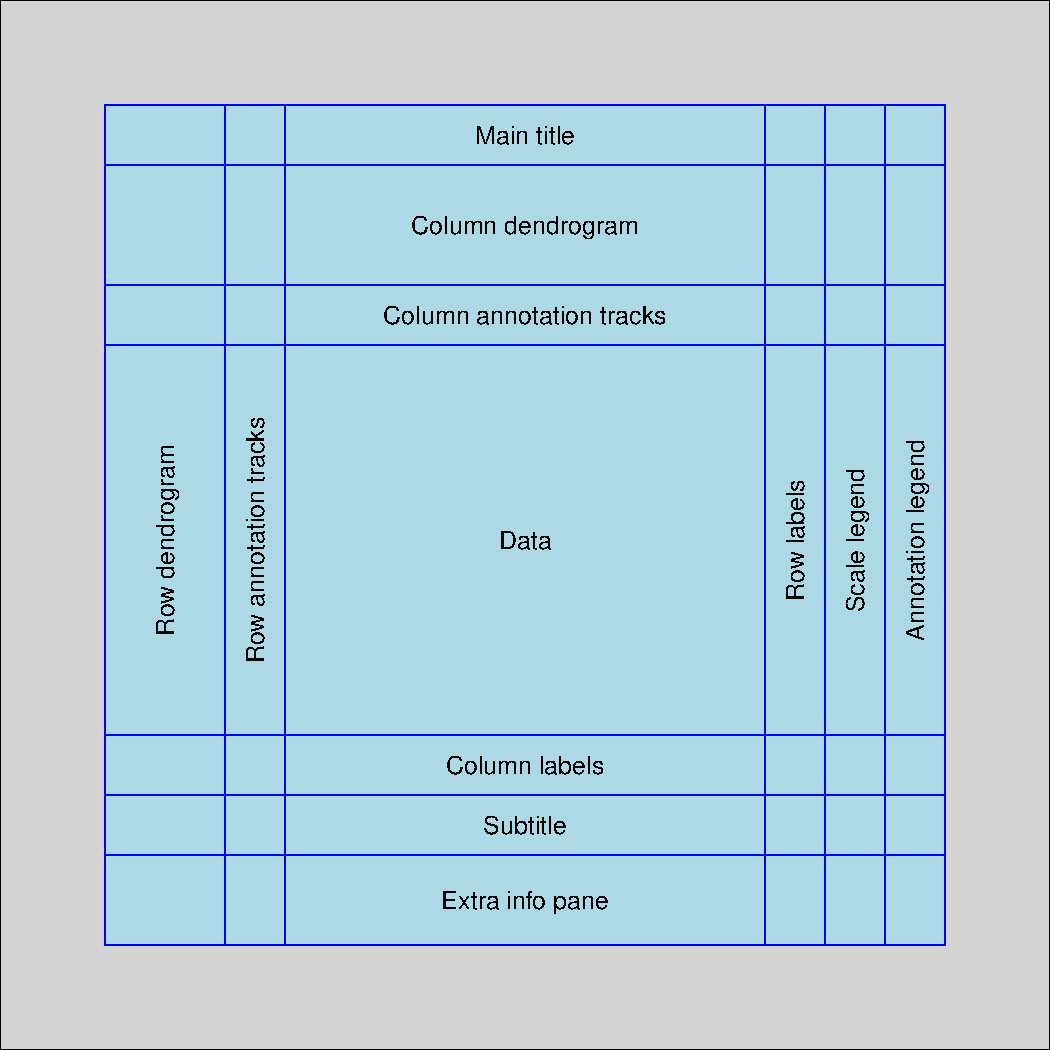
\includegraphics[width=.48\textwidth]{/home/renaud/Documents/projects/NMF/pkg/vignettes/figure/aheatmaps-layout1} 
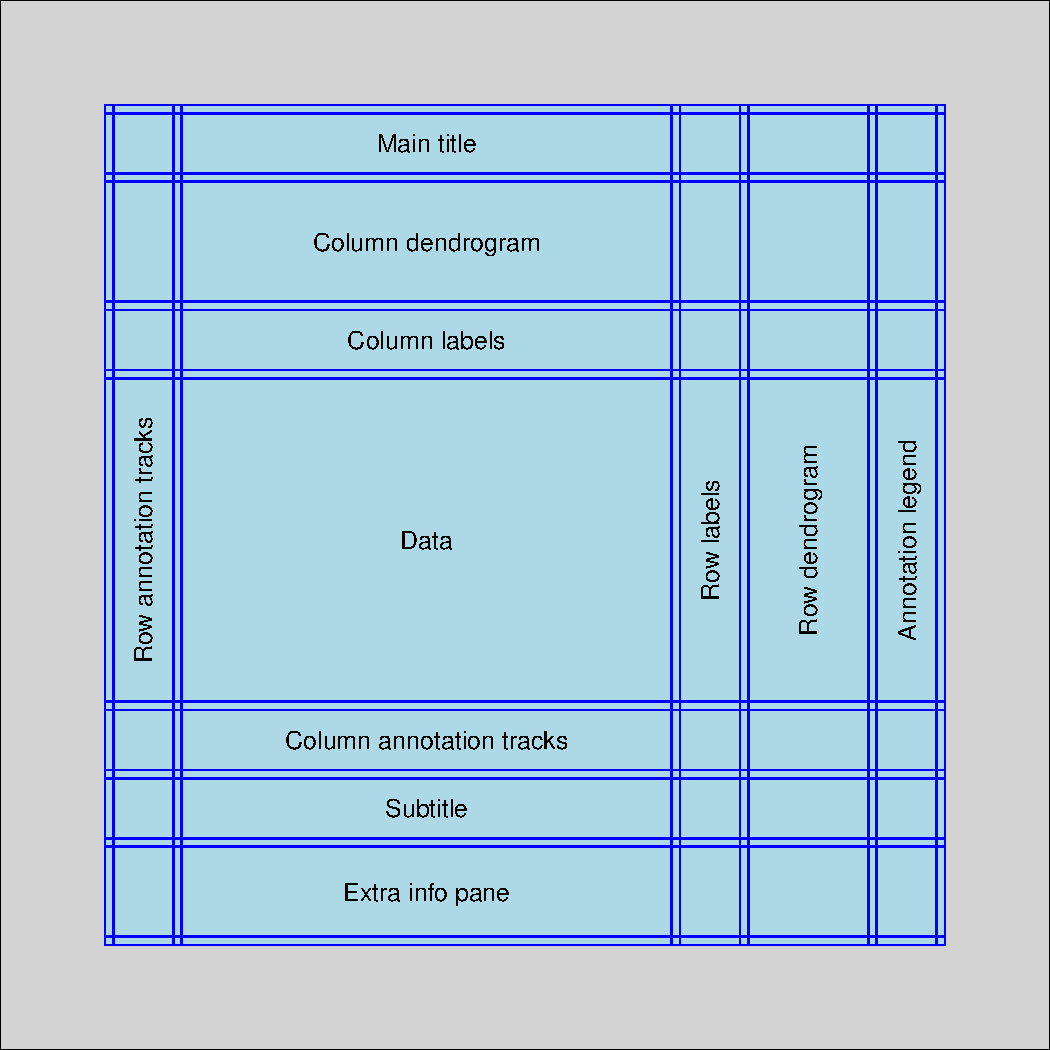
\includegraphics[width=.48\textwidth]{/home/renaud/Documents/projects/NMF/pkg/vignettes/figure/aheatmaps-layout2} 

\end{knitrout}

\caption{Grid layout diagram of annotated heatmaps: (left) default layout and
(right) an alternative layout, with separate specification for rows
and columns -- passed as a single string.}
\label{fig:layout}
\end{figure}

\section{Annotation tracks}
\section{Dendrograms}
\section{Column/row ordering}
\section{Colours}
\section{Labels}

\section{Legends}
Annotated heatmaps have two types of legends, one showing the colour-value scale
used to visualise the data matrix and another one for the annotation tracks.

\subsection{Colour scale}
The very principle of a heatmap is to bin the data values into a certain number
of intervals or breaks, and associate each of these with a given colour.
The colour scale is the legend that provides details about how to read the
resulting colour coded data matrix.
As such, it serves multiple purposes:
\begin{itemize}
  \item provide the mapping between colours and value intervals;
  \item show the actual range of displayed values;
  \item optionnaly show the overall distribution of values.
\end{itemize}

\subsubsection{Colours and breaks}

\subsubsection{Look and position}
As for other components in annotated heatmaps, the position of the
colour scale is controlled by the argument \code{layout}, which can also be used
to specify if the scale should be expand over the full height/width or have a
fixed size.

By default the scale is placed on the top-right corner of the data matrix, with
a fixed size.
\Cref{fig:layout_scale} illustrates how to obtain some other commonly used
positions/look.
However, more options are available, as detailed in the manual page for
\code{aheatmap\_layout}.

\begin{figure}[h!]
\begin{knitrout}\small
\definecolor{shadecolor}{rgb}{0.969, 0.969, 0.969}\color{fgcolor}\begin{kframe}
\begin{alltt}
\hlcom{# vertical on the right expanded over the full height}
\hlkwd{aheatmap}\hlstd{(x,} \hlkwc{layout} \hlstd{=} \hlstr{"*"}\hlstd{)}
\hlcom{# horizontal at the bottom-right corner}
\hlkwd{aheatmap}\hlstd{(x,} \hlkwc{layout} \hlstd{=} \hlstr{"_"}\hlstd{)}
\hlcom{# horizontal the bottom, expanded over the full width}
\hlkwd{aheatmap}\hlstd{(x,} \hlkwc{layout} \hlstd{=} \hlstr{"_*"}\hlstd{)}
\hlcom{# vertical on the left (when not using/showing row dendrogram)}
\hlkwd{aheatmap}\hlstd{(x,} \hlkwc{Rowv} \hlstd{=} \hlnum{NA}\hlstd{,} \hlkwc{layout} \hlstd{=} \hlstr{"L.|"}\hlstd{)}
\end{alltt}
\end{kframe}
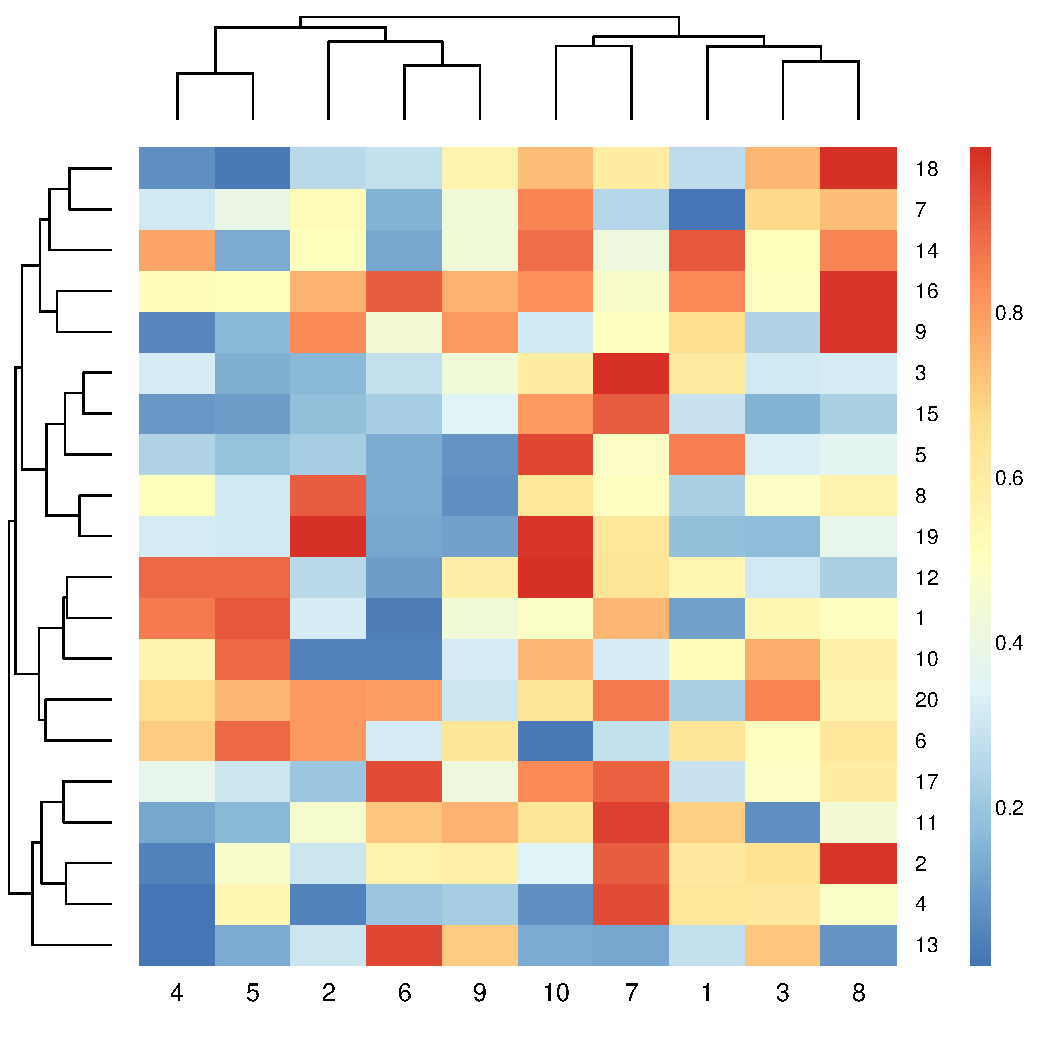
\includegraphics[width=0.25\textwidth]{/home/renaud/Documents/projects/NMF/pkg/vignettes/figure/aheatmaps-layout_scale1} 
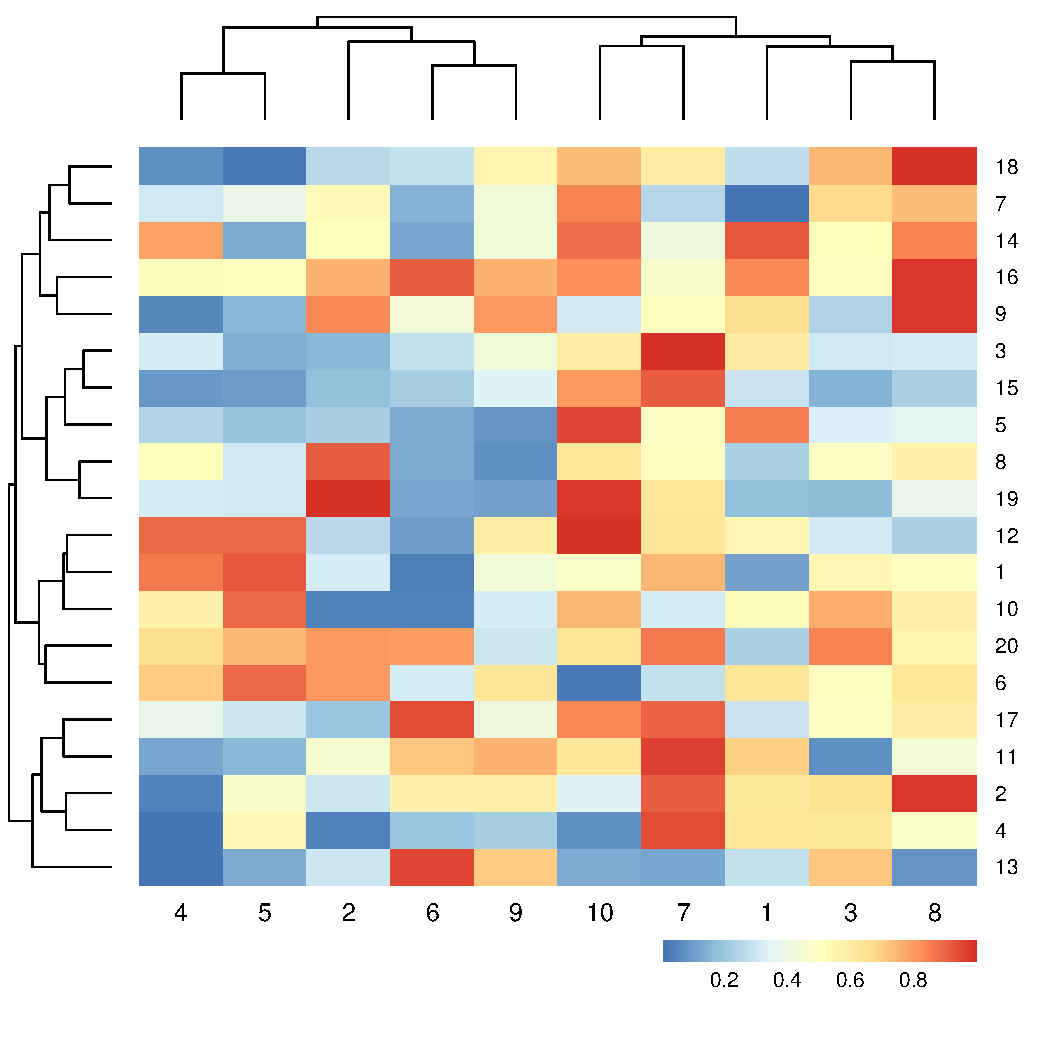
\includegraphics[width=0.25\textwidth]{/home/renaud/Documents/projects/NMF/pkg/vignettes/figure/aheatmaps-layout_scale2} 
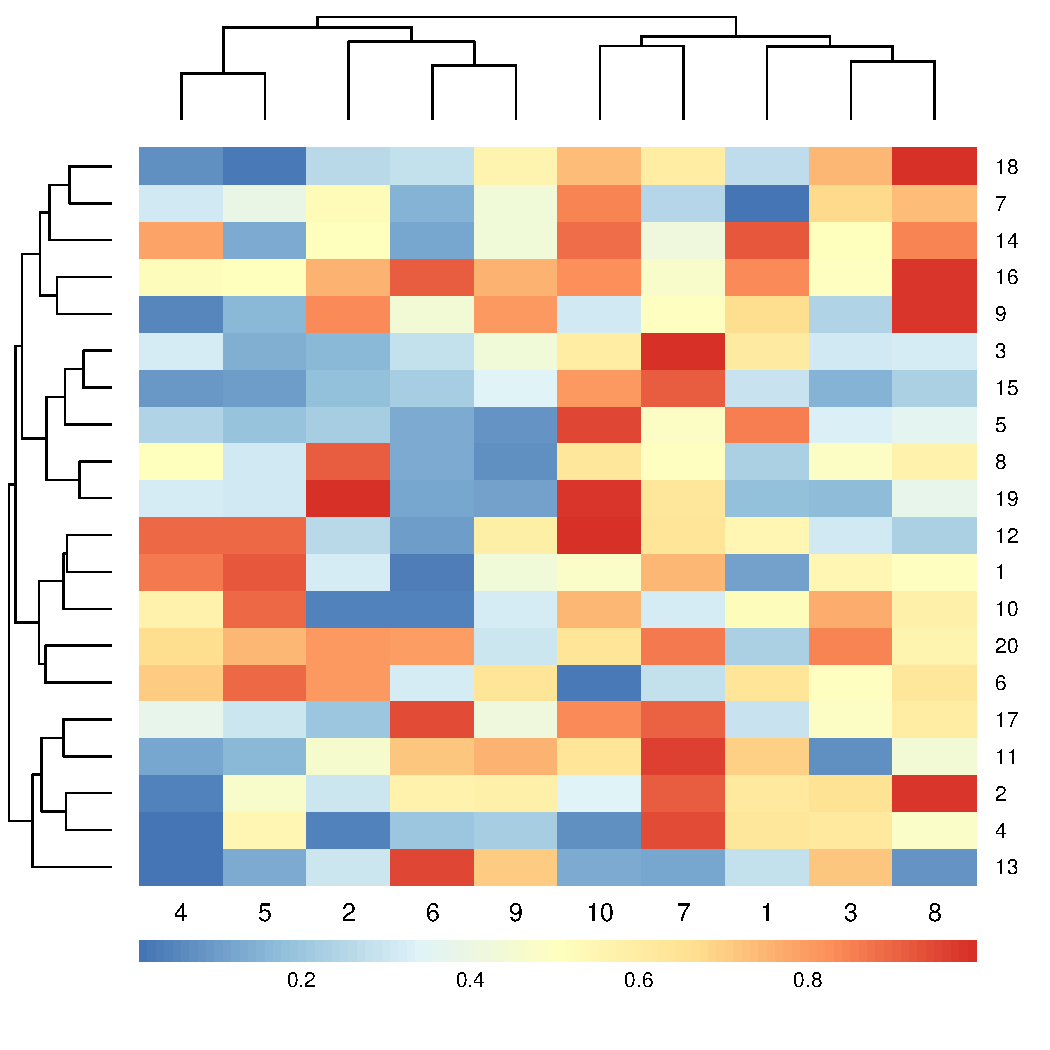
\includegraphics[width=0.25\textwidth]{/home/renaud/Documents/projects/NMF/pkg/vignettes/figure/aheatmaps-layout_scale3} 
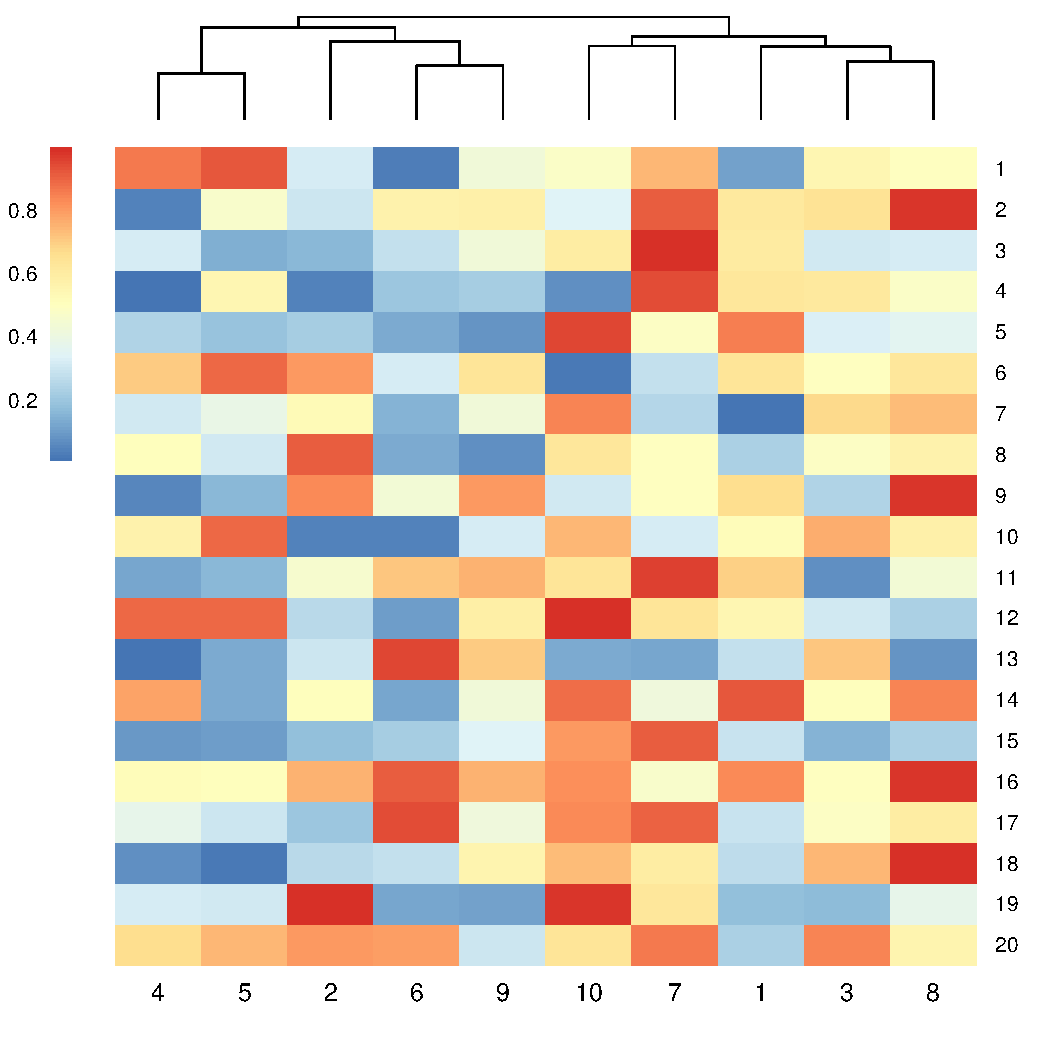
\includegraphics[width=0.25\textwidth]{/home/renaud/Documents/projects/NMF/pkg/vignettes/figure/aheatmaps-layout_scale4} 

\end{knitrout}

\caption{Colour scale alternative layouts: the scale can be placed in different
areas around the data matrix and expanded to full height/width.}
\label{fig:layout_scale}
\end{figure}


\subsection{Annotations}

\section{Session Info}
\begin{itemize}\raggedright
  \item R version 3.0.3 (2014-03-06), \verb|x86_64-pc-linux-gnu|
  \item Locale: \verb|LC_CTYPE=en_US.UTF-8|, \verb|LC_NUMERIC=C|, \verb|LC_TIME=en_US.UTF-8|, \verb|LC_COLLATE=en_US.UTF-8|, \verb|LC_MONETARY=en_US.UTF-8|, \verb|LC_MESSAGES=en_US.UTF-8|, \verb|LC_PAPER=en_US.UTF-8|, \verb|LC_NAME=C|, \verb|LC_ADDRESS=C|, \verb|LC_TELEPHONE=C|, \verb|LC_MEASUREMENT=en_US.UTF-8|, \verb|LC_IDENTIFICATION=C|
  \item Base packages: base, datasets, graphics, grDevices,
    methods, parallel, stats, utils
  \item Other packages: BH~1.51.0-4, bigmemory~4.4.6,
    bigmemory.sri~0.1.2, Biobase~2.22.0, BiocGenerics~0.8.0,
    cluster~1.15.1, knitr~1.5, NMF~0.21, pkgmaker~0.21,
    RColorBrewer~1.0-5, registry~0.2, rngtools~1.2.4,
    synchronicity~1.1.4
  \item Loaded via a namespace (and not attached):
    codetools~0.2-8, colorspace~1.2-4, dichromat~2.0-0,
    digest~0.6.4, doParallel~1.0.8, evaluate~0.5.1, foreach~1.4.1,
    formatR~0.10, ggplot2~0.9.3.1, grid~3.0.3, gridBase~0.4-7,
    gtable~0.1.2, highr~0.3, iterators~1.0.6, labeling~0.2,
    MASS~7.3-30, munsell~0.4.2, plyr~1.8.1, proto~0.3-10,
    Rcpp~0.11.1, reshape2~1.2.2, scales~0.2.3, stringr~0.6.2,
    tools~3.0.3, xtable~1.7-3
\end{itemize}



\printbibliography[heading=bibintoc]

\end{document}
